\documentclass[a4paper]{report}
\usepackage[utf8]{inputenc}
\usepackage[T1]{fontenc}
\title{Relatório - Representação de informação sonora}
\author{Ana Almeida e Pedro Alagoa}
\date{Maio 2014, Universidade de Aveiro}
\usepackage[portuguese]{babel}
\usepackage{indentfirst}
\usepackage[colorlinks=true,
            linkcolor=blue,
            urlcolor=blue,
            citecolor=red]{hyperref}
\usepackage{graphicx}
\usepackage{url}
\usepackage{tabularx}

%Glossário
\usepackage{glossaries}
\makeglossaries
\newglossaryentry{WAV}
{
    name=WAV, 
    description={ - WAVEform audio file format}
}
\newglossaryentry{MP3}
{
    name=MP3,
    description={ - abreviação de MPEG Layer 3, um formato de compressão de áudio digital.}
}
\newglossaryentry{AAC}
{
    name=AAC,
    description={ - abreviação de Advanced Audio Coding, um formato de compressão de áudio digital.}
}
\newglossaryentry{GSM}
{
    name=GSM,
    description={ - formato de áudio, muito utilizado em telemóveis.}
}
\newglossaryentry{bitrate}
{
    name=Bitrate, 
    description={ - n.º de bits convertidos/processados por unidade de tempo}
    plural=bitrates
}
\newglossaryentry{RMSD}
{
    name=RMSD,
    description={ - Root Mean Square Deviation(raiz quadrada da média do quadrado das diferenças}
}

\usepackage[procname]{listings}
\usepackage{color}

\definecolor{dkgreen}{rgb}{0,0.6,0}
\definecolor{gray}{rgb}{0.5,0.5,0.5}
\definecolor{mauve}{rgb}{0.58,0,0.82}

\definecolor{keywords}{RGB}{255,0,90}
\definecolor{comments}{RGB}{0,0,113}
\definecolor{red}{RGB}{160,0,0}
\definecolor{green}{RGB}{0,150,0}
 
 
\lstset{language=Python, 
        basicstyle=\ttfamily\small, 
        keywordstyle=\color{keywords},
        commentstyle=\color{comments},
        stringstyle=\color{red},
        showstringspaces=false,
        identifierstyle=\color{green},
        numbers=left,
        }

\bibliographystyle{unsrt}


\begin{document}
\begin{flushleft}
\begin{center}
 \Large{Universidade de Aveiro}
 \\[150pt]
 \fbox {\huge{Representação de informação sonora}}
 \\[75pt]
 \flushright{Ana Almeida}
 \\
 \flushright{Pedro Alagoa}
 \\[200pt]
 \flushleft \Large Relatório no âmbito de Laboratórios de Informática
 \\
 \flushright{Maio, 2014}
 \\
 Aveiro
\end{center} 

\maketitle

\begingroup
\hypersetup{linkcolor=black}
\tableofcontents
\endgroup
\clearpage

\cleardoublepage
\addcontentsline{toc}{section}{\listtablename}
\begingroup
\hypersetup{linkcolor=black}
\listoftables

\cleardoublepage
\addcontentsline{toc}{section}{\listfigurename}
\listoffigures
\endgroup

\clearpage

\end{flushleft}

\section{Resumo}
\label{resumo}

Com o intuito de comparar o resultado da codificação de ficheiros de áudio(\gls{MP3}, \gls{AAC} e \gls{GSM}) e, posteriormente, analisar os seus resultados, foi desenvolvida uma ferramenta utilizando o Python, onde são retirados valores como a gama dinâmica e o desvio entre o ficheiro codificado e o original.

Após a preparação da máquina e da instalação das aplicações e módulos necessários, procedeu-se à codificação do ficheiro modelo. De seguida, desenvolveu-se a ferramenta em Python e esta foi utilizada para retirar os valores pretendidos. Depois procedeu-se à sua análise, sob a forma de gráfico.

Ao analisar os gráficos obtidos, concluiu-se que, no geral, a codificação para \gls{MP3} é a mais indicada das 3 codificações, para os valores testados. A única excepção é no caso do \gls{GSM}, para \textit{bitrates} muito pequenos. Concluíu-se também que a gama dinâmica não é afectada pela variação de \textit{bitrates} de cada codec.

\chapter{Introdução}
\label{introducao}

Este relatório tem como objectivo principal aplicar as funcionalidades da linguagem Python no tratamento de informações de áudio.

Primeiramente, codificou-se um ficheiro de áudio de boa qualidade com codecs e valores de \gls{bitrate} diferentes. Depois, foram convertidos para \gls{WAV}, para serem processados pelo programa de Python.

O programa em Python servirá como uma ferramenta que compara o resultado da codificação, calculando a gama dinâmica e o desvio entre os valores do ficheiro final e do ficheiro original, que deverá ser obtido através do método \gls{RMSD}.

Por fim, este relatório conclui com um comentário final à análise dos resultados obtidos.

\chapter{Preparação}
\label{preparacao}

\section{Máquina e sistema operativo utilizados}
\label{machines}

A máquina utilizada foi o Toshiba Satellite P50-A-125.
O sistemas operativo utilizado foi o Windows 8 64 bit.

\section{Instalação das aplicações e módulos necessários}
\label{instalaraplicacoes}

Foi necessário instalar as seguintes aplicações: 
\begin{itemize}
\item {Python} v2.7.6 \cite{Python} 
\includegraphics[width=0.03\linewidth]{python_logo.png}
\item {Notepad++} v2.0.3\cite{Notepad++} 
\includegraphics[width=0.03\linewidth]{notepad++_logo.png}
\item {Audacity} v2.0.3\cite{Audacity} 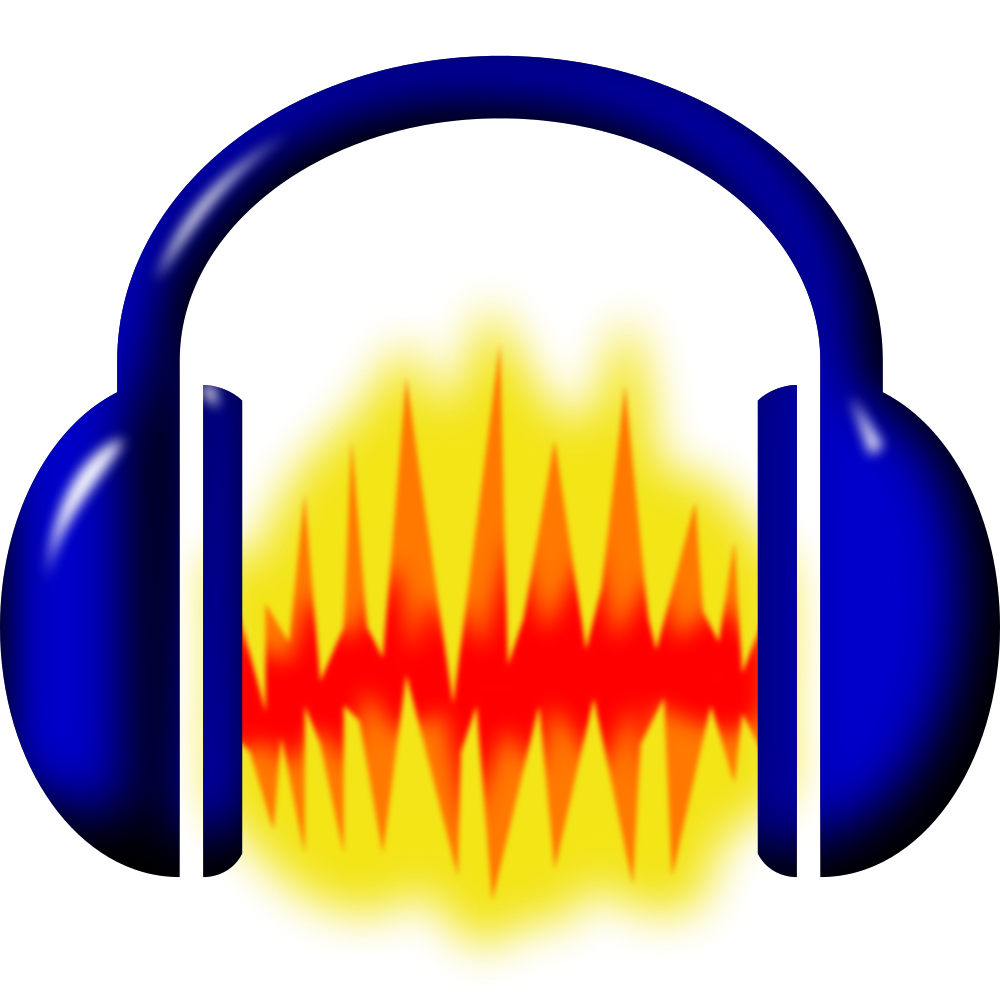
\includegraphics[width=0.03\linewidth]{audacity-logo.png}
\item {FDK AAC Encoder 0.5.3\cite{FDKACCEncoder} (libfdk-aac 3.4.12)}
\end{itemize}

Foi ainda necessário instalar alguns módulos necessários à implementação da ferramenta em Python. Os módulos instalados foram os seguintes:
\begin{itemize}
\item NumPy
\item SciPy
\end{itemize}

Como estes módulos não foram desenvolvidos para o sistema operativo em que se realizaram os testes, recorreu-se a \textit{binaries}\cite{Binaries} não oficiais.

O programa de reprodução de áudio utilizado foi o Foobar2000\cite{Foobar}.

\clearpage

\chapter{Procedimento}
\label{procedimento}

Depois de instalados e configurados os programas, procedeu-se à codificação do ficheiro de áudio em 3 formatos distintos: \gls{MP3}, \gls{AAC} e \gls{GSM}.

Procurou-se um ficheiro de áudio de alta qualidade e o escolhido foi uma música da autoria de ZUN, que faz parte da BGM do jogo Touhou 6\cite{TouhouProject}. O ficheiro de áudio utilizado pode ser obtido aqui: \url{http://wikisend.com/download/703922/th06_05.wav}.
\\[5pt]
O ficheiro utilizado tem as seguintes características:
\begin{description}
\item[Tipo de ficheiro] - WAV
\item[Tamanho] - 15,1 MB
\item[\textit{Bitrate}] - 1411kbps
\end{description}
\clearpage
\section{Codificação do ficheiro}
\label{codification}
\subsection{MP3}
\label{mp3codec}
Para codificar o ficheiro com codecs que originam um ficheiro \gls{MP3} utilizou-se o Audacity.

De seguida, como sugerido no enunciado do relatório, utilizou-se apenas um canal de áudio (mono).
\\
\begin{figure}[h!]
 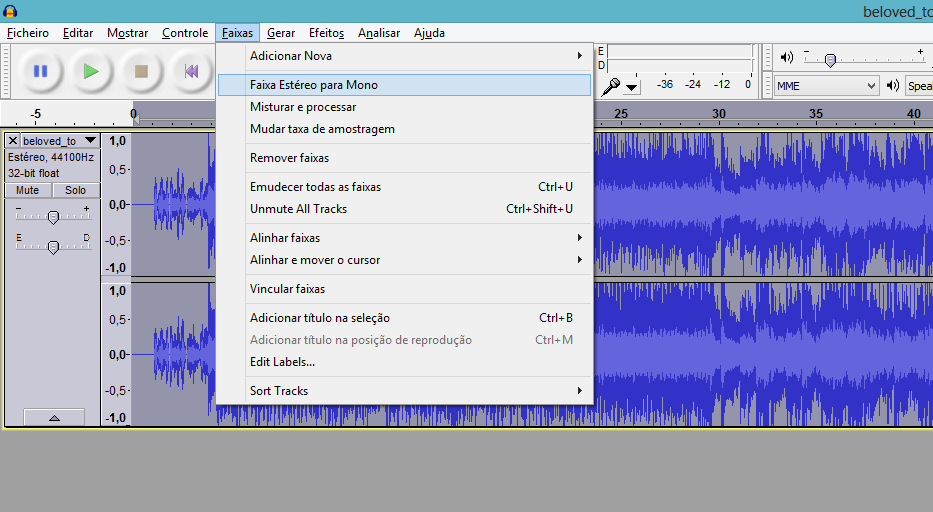
\includegraphics[width=\textwidth]{stereo_to_mono.png}
 \caption{Conversão de Stereo para Mono}
 \label{stereotomono}
\end{figure}


Depois procedeu-se à codificação do ficheiro, variando-se o valor de \gls{bitrate}. Ao todo, codificaram-se 6 ficheiros \gls{MP3}, com \textit{bitrates} de:
\begin{itemize}
\item 32kbps
\item 71kbps
\item 96kbps
\item 128kbps
\item 192kbps
\item 320kbps
\end{itemize}

Por fim, estes ficheiros foram convertidos para o formato \gls{WAV}, de modo a serem processados pela ferramenta implementada.

\subsection{AAC}
\label{aac}
Para codificar o ficheiro com codecs que originam um ficheiro \gls{AAC} utilizou-se a ferramenta FDK AAC Encoder 0.5.3, que utiliza a biblioteca de codecs fdk-aac.

Optou-se por utilizar esta aplicação porque a interface do Audacity não permite definir valores de \gls{bitrate} para os ficheiros \gls{AAC} e também porque o torna instável durante a reprodução do ficheiro.

Procedeu-se à codificação do ficheiro, variando-se o valor de \gls{bitrate}. Ao todo, codificaram-se 6 ficheiros \gls{AAC}, com bitrates de iguais aos codificados para o \gls{MP3} (ver \autoref{mp3codec}.)

\begin{figure}[ht]
 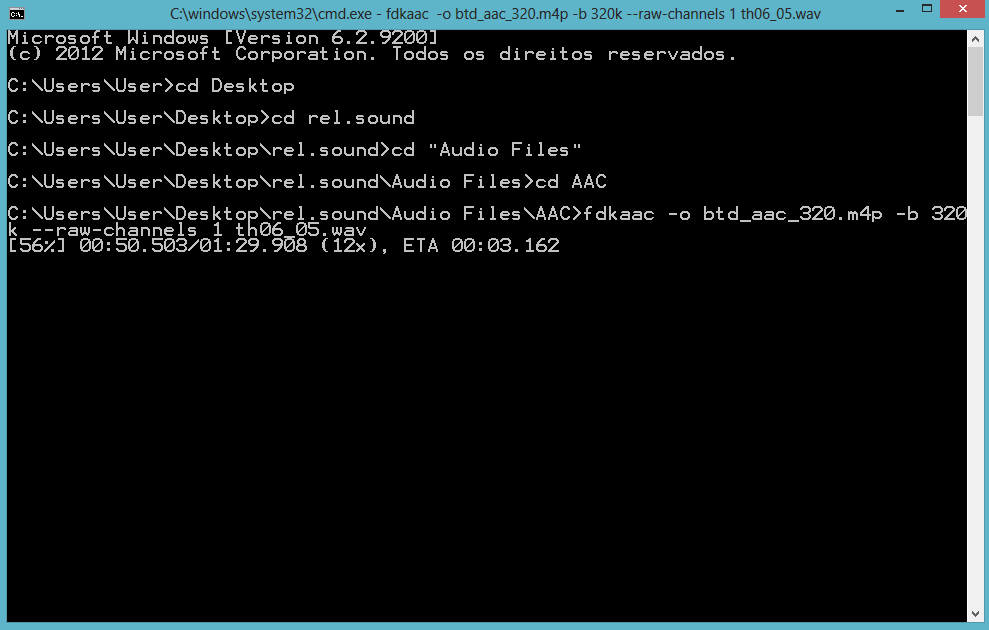
\includegraphics[width=\textwidth]{aac.png}
 \caption{FDK AAC Encoder em execução}
 \label{fdkaac}
\end{figure}

\begin{description}
\item[fdkaac] - Executa o programa
\item[-o btd\_aac\_320.m4p] - Nome do ficheiro de saída
\item[-b 320k] - Indica o \gls{bitrate} pretendido
\item[--raw-channels 1] - Indica o nº de canais a utilizar.
\item[th06\textunderscore05.wav] - Ficheiro de entrada.
\end{description}
De seguida, os ficheiros foram convertidos novamente para \gls{WAV}, utilizando o Audacity.

\subsection{GSM}
\label{gsm}
A codificação para \gls{GSM} só suporta um modo (71kbps), portanto só se obteve um ficheiro desse tipo.

Utilizou-se o Audacity para a conversão do ficheiro para \gls{GSM} e, posteriormente, para \gls{WAV}.
\section{Ferramenta em Python}
\label{pytool}
Para comparar os ficheiros obtidos, desenvolveu-se uma ferramenta em Python que calcula:
\begin{itemize}
\item A gama dinâmica.
\item O desvio entre os ficheiros codificados e o original, recorrendo a \gls{RMSD}.
\end{itemize}

A ferramenta recebe o nome de um ficheiro de áudio como argumento e quebra esse ficheiro em partes, cada uma contendo 1 frame. De seguida, lê o valor de cada parte, em dB, copiando-o para uma lista. Depois calcula valores, tais como o máximo, o mínimo, a gama dinâmica e o \gls{RMSD} em relação ao ficheiro original. Por fim, copia esses valores para um ficheiro de texto.

O código pode ser encontrado na integra na \autoref{pythontool}, onde existe também uma análise mais detalhada do mesmo.

\chapter{Análise de Resultados}
\label{analise}

\section{Gama Dinâmica}
\label{dinamicrange}
A gama dinâmica é o rácio entre o valor máximo e mínimo obtido. No caso dos dB, é uma escala que contém valores negativos. Portanto este rácio funciona da seguinte forma: 
\begin{description}
\item[Se é positivo] - Quanto maior for o rácio, maior será a gama dinâmica (e vice-versa).
\item [Se é negativo] - Quanto menor for o rácio, maior será a gama dinâmica (e vice-versa).
\end{description}

As gamas dinâmicas obtidas foram comparadas em forma de gráfico de barras.

\begin{figure}[ht]
 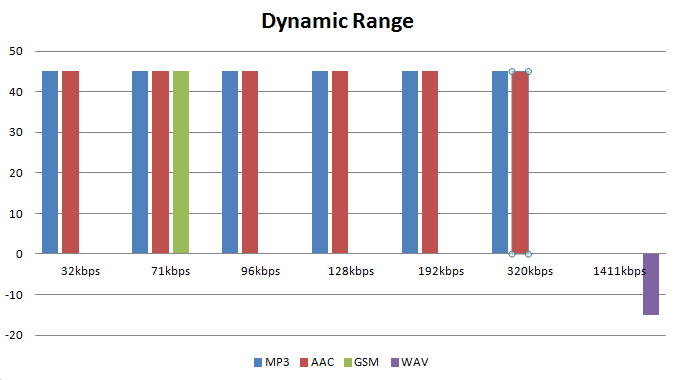
\includegraphics[width=\textwidth]{dr.png}
 \caption{Gama Dinâmica}
 \label{dr}
\end{figure}

Pode-se observar que, nos ficheiros codificados, a gama dinâmica é igual para todos os ficheiros. Porém, é diferente do ficheiro original, que, como possui valores de dB negativos, tem uma gama dinâmica superior.

\section{RMSD}

A raíz quadrada da média do quadrado das diferenças é um método de calcular a diferença entre valores esperados e valores obtidos. 

Quanto menor for o \gls{RMSD}, mais proximo estará o ficheiro do original.
\\
\begin{figure}[ht]
 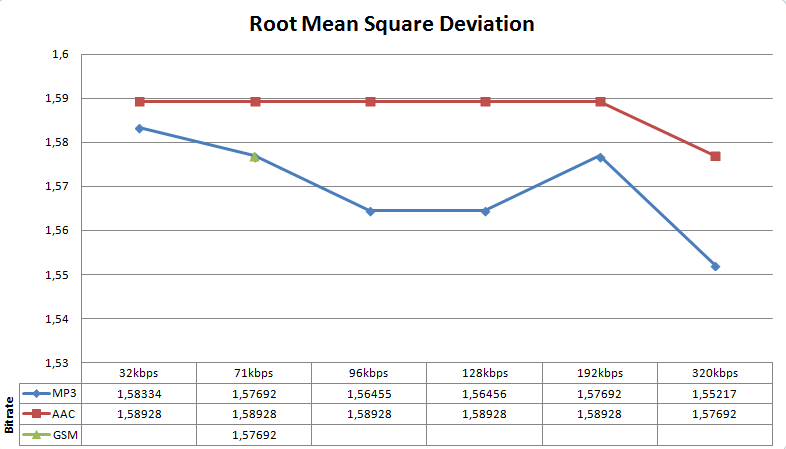
\includegraphics[width=\textwidth]{rmsd.png}
 \caption{RMSD}
 \label{rmsd}
\end{figure}

Ao observar o \autoref{rmsd}, verifica-se que os ficheiros \gls{MP3} são mais próximos que o original, no que toca aos valores tidos em conta.

Observa-se ainda que, para \textit{bitrates} baixos, os ficheiros \gls{AAC} não se tornam mais próximos do original, sendo o \gls{RMSD} igual, excepto para o ficheiro codificado a 320kbps.

Verifica-se também que o ficheiro \gls{GSM} é tão próximo do original como o \gls{MP3} com \gls{bitrate} correspondente.

\section{Tamanho do ficheiro}
\label{filesize}
Foi também verificado o tamanho dos ficheiros \gls{MP3}, \gls{AAC} e \gls{GSM}.
\\[5pt]

\begin{table}[h]
 \begin{center}
  \begin{tabularx}{\textwidth}{|X|X|X|X|X|X|X|}
    \hline 
            & 32kbps & 71kbps & 96kbps & 128kbps & 192kbps & 320kbps \\ 
    \hline 
        MP3 & 352KB & 879KB & 1055KB & 1406KB & 2109KB & 3515KB \\ 
    \hline 
        AAC & 370KB & 798KB & 1072KB & 1423KB & 2126KB & 3531KB \\ 
    \hline 
        GSM & - & 787KB & - & - & - & - \\ 
    \hline 
  \end{tabularx} \\
  \vspace{-5pt}
  \caption{Tamanhos dos ficheiros}
  \label{size}
 \end{center}
\end{table}

Podemos verificar na \autoref{size} que os ficheiros \gls{MP3}, no geral, são mais pequenos que os ficheiros \gls{AAC}.

No caso em que o \gls{GSM} está presente, o ficheiro que tem menor tamanho é o \gls{GSM}.

O ficheiro original(WAV) tem 15,1MB, como já referido no \autoref{procedimento}.
\chapter{Conclusão}
\label{conclusion}

Comparando os resultados, obtemos as seguintes conclusões:
\begin{itemize}
\item A gama dinâmica não é afectada, no que diz respeito à variação de \gls{bitrate}.
\item Os ficheiros \gls{MP3} são mais recomendados que os \gls{AAC} para todos os \textit{bitrates}, uma vez que são mais próximos do ficheiro original e ligeiramente mais pequenos.
\item Quando se trata de \textit{bitrates} muito pequenos (na ordem dos 71kbps), os ficheiros \gls{GSM} são melhores, uma vez que oferecem a mesma qualidade que os \gls{MP3}, ocupando muito menos espaço.
\end{itemize}

\clearpage

\addcontentsline{toc}{chapter}{Glossário}
\renewcommand*{\glossaryname}{Glossário}
\printglossaries

\clearpage
\addcontentsline{toc}{chapter}{Bibliografia}
\bibliography{references}


\appendix
\chapter{Comparador}
\label{pythontool}
\section{Código}
\label{code}
\lstinputlisting[language=Python]{comparator.py}
\section{Descrição}
\label{description}
\begin{description}
\item[1-5] - Importação dos módulos necessários.
\item[6-9] - Abertura dos ficheiros WAVE com os módulos wave e scipy.
\item[11-13] - O ficheiro é quebrado em pedaços (1 frame por pedaço)
\item[14-16] - Os valores de dB dos respectivos frames são retirados para uma lista.
\item[18-41] - Os valores pretendidos são calculados, percorrendo a lista com os dBs.
\item[41] - O valor 38.845891991 corresponde ao valor RMS do ficheiro original, que foi obtido através do código presente na \autoref{tool}
\item[42-51] - É criada uma lista de Strings, que vão ser copiadas para um ficheiro de texto.
\item[53-55] - A lista é copiada para o ficheiro.

\end{description}

\chapter{Ferramenta}
\label{tool}
\lstinputlisting[language=Python]{tool.py}

\end{document}
    